% !TeX program = xelatex
\ifdefined\BookMaster\else
\documentclass[11pt,oneside]{article}
% !TeX program = xelatex
\usepackage[b5paper,left=22mm,right=22mm,top=20mm,bottom=22mm,footskip=11mm]{geometry}
\usepackage{fontspec}
\setmainfont{TeX Gyre Termes}
\setsansfont{TeX Gyre Heros}
\usepackage{amsmath,amssymb,mathtools,amsthm}
\renewcommand{\cdots}{\mathinner{\cdotp\cdotp\cdotp}}
\usepackage{graphicx,adjustbox,array,booktabs,longtable,multirow,enumitem,changepage,needspace}
\usepackage[table]{xcolor}
\usepackage{fancyhdr}
\raggedbottom
\interfootnotelinepenalty=10000
\newcommand{\BookFootnote}[2]{\begingroup\renewcommand{\thefootnote}{\fnsymbol{footnote}}\footnote[#1]{#2}\endgroup}
\newcommand{\BookFootnoteMark}[1]{\begingroup\renewcommand{\thefootnote}{\fnsymbol{footnote}}\footnotemark[#1]\endgroup}
\newcommand{\BookFootnoteText}[2]{\begingroup\renewcommand{\thefootnote}{\fnsymbol{footnote}}\footnotetext[#1]{#2}\endgroup}
\newenvironment{BookFloat}[1]{\par\addvspace{.6\baselineskip}\noindent\def\BookFloatID{#1}\begin{minipage}{\linewidth}\phantomsection\label{bookfloat:#1:start}}{\phantomsection\label{bookfloat:\BookFloatID:end}\end{minipage}\par\addvspace{.6\baselineskip}}

\usepackage[unicode,hidelinks]{hyperref}
\pagestyle{fancy}
\fancyhf{}
\newcommand{\BookFooter}{}
\fancyfoot[L]{\parbox[b]{\dimexpr\textwidth-15mm}{\footnotesize\BookFooter}}
\fancyfoot[R]{\footnotesize\thepage}
\renewcommand{\headrulewidth}{0pt}
\renewcommand{\footrulewidth}{0pt}
\setlength{\parindent}{0pt}
\setlength{\parskip}{0.2em}
\setlength{\emergencystretch}{3em}
\setlist{nosep,leftmargin=1.7em,labelsep=.65em}
\newif\ifBookNarrative
\BookNarrativetrue
\newenvironment{BookBody}{\setlength{\parindent}{0pt}}{}
\newcommand{\BookStatement}[1]{\par\addvspace{.6\baselineskip}\noindent #1\enspace\ignorespaces}
\newcommand{\BookLabel}[1]{\par\addvspace{.6\baselineskip}\needspace{3\baselineskip}\noindent\textbf{#1}\quad\ignorespaces}
\newcommand{\BookHeading}[1]{\par\addvspace{\baselineskip}\needspace{4\baselineskip}\noindent{\large\bfseries #1}\par\medskip}
\newcommand{\BookSubheading}[1]{\par\addvspace{.7\baselineskip}\needspace{3\baselineskip}\noindent{\bfseries #1}\par\smallskip}
\newcommand{\BookTextHeading}[1]{\par\addvspace{.7\baselineskip}\needspace{3\baselineskip}\noindent #1\par\smallskip}
\newcommand{\BookSectionTitle}[2]{\par\addvspace{1.2\baselineskip}\needspace{5\baselineskip}\noindent\colorbox{gray!25}{\sffamily\bfseries\small SECTION #1}\quad{\large\bfseries #2}\par\medskip}
\newcommand{\BookExerciseTitle}[1]{\par\addvspace{\baselineskip}\needspace{4\baselineskip}\noindent{\color{gray}\rule{1.5mm}{1.5mm}}\enspace{\large\bfseries Exercises #1}\par\medskip}
\newcommand{\BookBullet}[1]{\begin{list}{\textbullet}{\setlength{\leftmargin}{1.7em}\setlength{\labelwidth}{1em}\setlength{\labelsep}{.7em}\setlength{\topsep}{0pt}\setlength{\parsep}{0pt}\setlength{\itemsep}{0pt}}\item #1\end{list}}
\newcommand{\BookExercise}[2]{\begin{list}{\textbf{#1}}{\setlength{\leftmargin}{2.2em}\setlength{\labelwidth}{1.5em}\setlength{\labelsep}{.7em}\setlength{\topsep}{.15em}\setlength{\parsep}{0pt}\setlength{\itemsep}{0pt}}\item #2\end{list}}
\newcommand{\BookEnd}[1]{\unskip\nobreak\hfill\ensuremath{#1}}
\newcommand{\BookSource}[2]{\phantomsection\label{sourcepage:#1}} % Source-page anchors, retained through reflow.
\usepackage{multicol}
\usepackage{tikz}
\newcommand{\BookPartEntry}[2]{\par\noindent\makebox[17mm][l]{\bfseries Section #1}#2\par}
\newcommand{\BookPartTitle}[3]{\par\bigskip\noindent\begin{tikzpicture}\node[anchor=north west,inner sep=0pt,outer sep=0pt] (bookpart) at (0,0) {\begin{minipage}{\dimexpr\linewidth-.5pt}\hspace*{26mm}\begin{minipage}[t]{\dimexpr\linewidth-26mm}\begin{adjustbox}{max width=\linewidth}{\fontsize{20}{24}\selectfont\bfseries #2}\end{adjustbox}\par\vspace{6mm}\hrule\vspace{6mm}{\sffamily\footnotesize\setlength{\parskip}{.3em}#3}\vspace{3mm}\end{minipage}\end{minipage}};\path[shade,top color=gray!60,bottom color=white] (0,0) rectangle ([xshift=24mm]bookpart.south west);\node[anchor=north,font=\sffamily\bfseries\small] at (12mm,-2mm) {PART};\node[anchor=north,font=\sffamily\bfseries\Huge] at (12mm,-7mm) {#1};\end{tikzpicture}\par\bigskip}
\newsavebox{\BookMathBox}
\makeatletter
\newcommand{\BookInline}[1]{\leavevmode\hskip0pt\relax\begingroup\in@{\begin}{#1}\ifin@\sbox{\BookMathBox}{\(#1\)}\ifdim\wd\BookMathBox>\dimexpr\linewidth-1em\relax\resizebox{\dimexpr\linewidth-1em\relax}{!}{\usebox{\BookMathBox}}\else\(#1\)\fi\else\in@{\left}{#1}\ifin@\sbox{\BookMathBox}{\(#1\)}\ifdim\wd\BookMathBox>\dimexpr\linewidth-1em\relax\resizebox{\dimexpr\linewidth-1em\relax}{!}{\usebox{\BookMathBox}}\else\(#1\)\fi\else\(#1\)\fi\fi\endgroup\hskip0pt\relax}
\makeatother
\DeclareMathOperator{\Aut}{Aut}
\DeclareMathOperator{\End}{End}
\DeclareMathOperator{\Hom}{Hom}
\DeclareMathOperator{\GF}{GF}
\DeclareMathOperator{\irr}{irr}
\DeclareMathOperator{\lt}{lt}
\DeclareMathOperator{\lp}{lp}
\providecommand{\textcircled}[1]{\textnormal{(#1)}}

\begin{document}
\fi
\renewcommand{\BookFooter}{Section 47 Illustrations of Galois Theory}
\pdfbookmark[0]{Section 47 Illustrations of Galois Theory}{47_illustrations_of_galois_theory}
\ifdefined\BookMaster\else\setcounter{page}{372}\fi
% Source PDF page 389; original printed page 372
\BookSource{389}{372}
\BookNarrativetrue

\begin{BookBody}

\BookSectionTitle{47}{Illustrations of Galois Theory}

\BookTextHeading{\textbf{Symmetric Functions}  }

\noindent Let \BookInline{F} be a field of characteristic zero, and let \BookInline{y_{1},\allowbreak \cdots,\allowbreak y_{n}} be indeterminates. There are some natural automorphisms of \BookInline{F(y_{1},\allowbreak \cdots,\allowbreak y_{n})} leaving \BookInline{F} fixed, namely, those defined by permutations of \BookInline{\{y_{1},\allowbreak \cdots,\allowbreak y_{n}\}.} To be more explicit, let \BookInline{\sigma } be a permutation of \BookInline{\{1,\allowbreak \cdots,\allowbreak n\},\allowbreak } that is\BookInline{,\allowbreak \sigma \in S_{n}.} Then \BookInline{\sigma } gives rise to a natural map \BookInline{\sigma:F(y_{1},\allowbreak \cdots,\allowbreak y_{n})\to F(y_{1},\allowbreak \cdots,\allowbreak y_{n})} given by

\begin{center}\begin{adjustbox}{max width=\linewidth}\BookInline{\displaystyle \overline { { \sigma } } \left( \frac { f ( y _ { 1 } ,\allowbreak  \cdots ,\allowbreak  y _ { n } ) } { g ( y _ { 1 } ,\allowbreak  \cdots ,\allowbreak  y _ { n } ) } \right) = \frac { f ( y _ { \sigma ( 1 ) } ,\allowbreak  \cdots ,\allowbreak  y _ { \sigma ( n ) } ) } { g ( y _ { \sigma ( 1 ) } ,\allowbreak  \cdots ,\allowbreak  y _ { \sigma ( n ) } ) }}\end{adjustbox}\end{center}

\noindent for \BookInline{f(y_{1},\allowbreak \cdots,\allowbreak y_{n}),\allowbreak g(y_{1},\allowbreak \cdots,\allowbreak y_{n})\in F[y_{1},\allowbreak \cdots,\allowbreak y_{n}],\allowbreak } with \BookInline{g(y_{1},\allowbreak \cdots,\allowbreak y_{n})\neq 0.} It is immediate that \BookInline{\overline{\sigma }} is an automorphism of \BookInline{F(y_{1},\allowbreak \cdots,\allowbreak y_{n})} leaving \BookInline{F} fixed. The elements of \BookInline{F(y_{1},\allowbreak \cdots,\allowbreak y_{n})} left fixed by\textit{ all} \BookInline{\overline{\sigma },\allowbreak } for all \BookInline{\sigma \in S_{n},\allowbreak } are those rational functions that are \textit{symmetric} in the indeterminates \BookInline{y_{1},\allowbreak \cdots,\allowbreak y_{n}.}

\BookLabel{47.1 Definition} An element of the field \BookInline{F(y_{1},\allowbreak \cdots,\allowbreak y_{n})} is a\textbf{ symmetric function in} \BookInline{y_{1},\allowbreak \cdots,\allowbreak y_{n}} \textbf{over} \BookInline{F,\allowbreak } if it is fixed by all permutations of \BookInline{y_{1},\allowbreak \cdots,\allowbreak y_{n},\allowbreak } in the sense just explained\BookInline{.}\BookEnd{\blacksquare}

Let \BookInline{\overline{S_{n}}} be the group of all the automorphisms \BookInline{\overline{\sigma }} for \BookInline{\sigma \in S_{n}.} Observe that \BookInline{\overline{S_{n}}} is naturally isomorphic to \BookInline{S_{n}.} Let \BookInline{K} be the subfield of \BookInline{F(y_{1},\allowbreak \cdots,\allowbreak y_{n}),\allowbreak } which is the fixed field of \BookInline{\overline{S_{n}}.} Consider the polynomial

\begin{center}\begin{adjustbox}{max width=\linewidth}\BookInline{\displaystyle f(x)= \prod _{i= 1}^{n}(x- y_{i});}\end{adjustbox}\end{center}

\noindent this polynomial \BookInline{f(x)\in (F(y_{1},\allowbreak \cdots,\allowbreak y_{n}))[x]} is a\textbf{ general polynomial of degree} \BookInline{n.} Let \BookInline{\overline{\sigma _{x}}} be the polynomial extension of \BookInline{\overline{\sigma },\allowbreak } as defined in Definition 44.4, to \BookInline{(F(y_{1},\allowbreak \cdots,\allowbreak y_{n}))[x],\allowbreak } where \BookInline{\overline{\sigma _{x}}(x)= x.} Now \BookInline{f(x)} is fixed by each map \BookInline{\overline{\sigma _{x}}} for \BookInline{\sigma \in S_{n};} that is,

\begin{center}\begin{adjustbox}{max width=\linewidth}\BookInline{\displaystyle \prod _{i= 1}^{n}(x- y_{i})= \prod _{i= 1}^{n}(x- y_{\sigma (i)}).}\end{adjustbox}\end{center}

\noindent Thus the coefficients of \BookInline{f(x)} are in \BookInline{K;} they are, except for sign, the\textit{ elementary symmetric} \textit{functions} in \BookInline{y_{1},\allowbreak \cdots,\allowbreak y_{n}.} As illustration, note that the constant term of \BookInline{f(x)} is

\begin{center}\begin{adjustbox}{max width=\linewidth}\BookInline{\displaystyle (- 1)^{n}y_{1}y_{2}\cdots y_{n},\allowbreak }\end{adjustbox}\end{center}

\noindent the coefficient of \BookInline{x^{n- 1}} is \BookInline{- (y_{1}+ y_{2}+ \cdots + y_{n}),\allowbreak } and so on. These are symmetric functions in \BookInline{y_{1},\allowbreak \cdots,\allowbreak y_{n}.}

The first elementary symmetric function in \BookInline{y_{1},\allowbreak \cdots,\allowbreak y_{n}} is

\begin{center}\begin{adjustbox}{max width=\linewidth}\BookInline{\displaystyle s_{1}= y_{1}+ y_{2}+ \cdots + y_{n},\allowbreak }\end{adjustbox}\end{center}

\noindent the second is \BookInline{s_{2}= y_{1}y_{2}+ y_{1}y_{3}+ \cdots + y_{n- 1}y_{n},\allowbreak } and so on, and the \BookInline{n}th is \BookInline{s_{n}= y_{1}y_{2}\cdots y_{n}.} Consider the field \BookInline{E= F(s_{1},\allowbreak \cdots,\allowbreak s_{n}).} Of course\BookInline{,\allowbreak E\leq K,\allowbreak } where \BookInline{K} is the field of all symmetric functions in \BookInline{y_{1},\allowbreak \cdots,\allowbreak y_{n}} over \BookInline{F.} Since the characteristic of \BookInline{E} is zero, the extension \BookInline{K} over \BookInline{E} is a separable extension. Thus \BookInline{F(y_{1},\allowbreak \cdots,\allowbreak y_{n})} is a finite normal extension of \BookInline{E,\allowbreak } namely, the splitting field of

\begin{center}\begin{adjustbox}{max width=\linewidth}\BookInline{\displaystyle f(x)= \prod _{i= 1}^{n}(x- y_{i})}\end{adjustbox}\end{center}

\noindent over \BookInline{E.} Since the degree of \BookInline{f(x)} is \BookInline{n,\allowbreak } we have at once that

\begin{center}\begin{adjustbox}{max width=\linewidth}\BookInline{\displaystyle [F(y_{1},\allowbreak \cdots ,\allowbreak y_{n}):E]\leq n!}\end{adjustbox}\end{center}

\end{BookBody}

% Source PDF page 390; original printed page 373
\BookSource{390}{373}
\BookNarrativetrue

\begin{BookBody}

\noindent (see Exercise 19, Section 44). However, since \BookInline{K} is the fixed field of \BookInline{\overline{S_{n}}} and

\begin{center}\begin{adjustbox}{max width=\linewidth}\BookInline{\displaystyle |\overline{S_{n}}|= |S_{n}|= n!,\allowbreak }\end{adjustbox}\end{center}

\noindent we have also

\begin{center}\begin{adjustbox}{max width=\linewidth}\BookInline{\displaystyle n!= [F(y_{1},\allowbreak \cdots ,\allowbreak y_{n}):K].}\end{adjustbox}\end{center}

\noindent Therefore,

\begin{center}\begin{adjustbox}{max width=\linewidth}\BookInline{\displaystyle n!= [F(y_{1},\allowbreak \cdots ,\allowbreak y_{n}):K]\leq [F(y_{1},\allowbreak \cdots ,\allowbreak y_{n}):E]\leq n!,\allowbreak }\end{adjustbox}\end{center}

\noindent so

\begin{center}\begin{adjustbox}{max width=\linewidth}\BookInline{\displaystyle K= E.}\end{adjustbox}\end{center}

\noindent The full Galois group of \BookInline{F(y_{1},\allowbreak \cdots,\allowbreak y_{n})} over \BookInline{E} is therefore \BookInline{\overline{S_{n}}.} The fact that \BookInline{K= E} shows that every symmetric function can be expressed as a rational function of the elementary symmetric functions \BookInline{s_{1},\allowbreak \cdots,\allowbreak s_{n}.} We summarize these results in a theorem.

\BookLabel{47.2 Theorem} Let \BookInline{F} be a field with characteristic zero. Let \BookInline{s_{1},\allowbreak \cdots,\allowbreak s_{n}} be the elementary symmetric functions in the indeterminates \BookInline{y_{1},\allowbreak \cdots,\allowbreak y_{n}.} Then every symmetric function of \BookInline{y_{1},\allowbreak \cdots,\allowbreak y_{n}} over \BookInline{F} is a rational function of the elementary symmetric functions. Also\BookInline{,\allowbreak F(y_{1},\allowbreak \cdots,\allowbreak y_{n})} is a finite normal extension of degree \BookInline{n!} of \BookInline{F(s_{1},\allowbreak \cdots,\allowbreak s_{n}),\allowbreak } and the Galois group of this extension is naturally isomorphic to \BookInline{S_{n}.}

In view of Cayley’s Theorem 8.11, it can be deduced from Theorem 47.2 that any finite group can occur as a Galois group (up to isomorphism). (See Exercise 11.)

The proof of Theorem 47.2 only uses the fact that the characteristic of \BookInline{F} is zero to conclude that the extension \BookInline{F(y_{1},\allowbreak y_{2},\allowbreak...,\allowbreak y_{n})} over \BookInline{E} is a separable extension. With a bit more work, the proof can be modified to allow \BookInline{F} to be an arbitrary field.

\BookTextHeading{\textbf{Examples}}

\noindent Let us give our promised example of a finite normal extension having a Galois group whose subgroup diagram does not look like its own inversion.

\BookLabel{47.3 Example} Consider the splitting field in \BookInline{\mathbb{C}} of \BookInline{x^{4}- 2} over \BookInline{\mathbb{Q}.} Now \BookInline{x^{4}- 2} is irreducible over \BookInline{\mathbb{Q},\allowbreak } by Eisenstein’s criterion, with \BookInline{p= 2.} Let \BookInline{\alpha = \sqrt [ 4 ] { 2 }} be the real positive zero of \BookInline{x^{4}- 2.} Then the four zeros of \BookInline{x^{4}- 2} in \BookInline{\mathbb{C}} are \BookInline{\alpha,\allowbreak - \alpha,\allowbreak i\alpha,\allowbreak } and \BookInline{- i\alpha,\allowbreak } where \BookInline{i} is the usual zero of \BookInline{x^{2}+ 1} in \BookInline{\mathbb{C}.} The splitting field \BookInline{K} of \BookInline{x^{4}- 2} over \BookInline{\mathbb{Q}} thus contains \BookInline{(i\alpha )/\alpha = i.} Since \BookInline{\alpha } is a real number\BookInline{,\allowbreak \mathbb{Q}(\alpha )<\mathbb{R},\allowbreak } so \BookInline{\mathbb{Q}(\alpha )\neq K.} However, since \BookInline{\mathbb{Q}(\alpha,\allowbreak i)} contains all zeros of \BookInline{x^{4}- 2,\allowbreak } we see that \BookInline{\mathbb{Q}(\alpha,\allowbreak i)= K.} Letting \BookInline{E= \mathbb{Q}(\alpha ),\allowbreak } we have the diagram in Fig. 47.4.

\begin{BookFloat}{47_illustrations_of_galois_theory-p390-15}
\begin{center}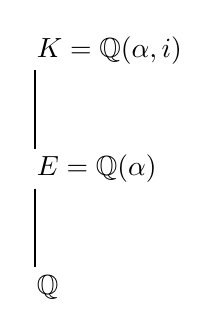
\begin{tikzpicture}
\node[anchor=west] (K) at (0,3) {$K=\mathbb{Q}(\alpha,i)$};
\node[anchor=west] (E) at (0,1.5) {$E=\mathbb{Q}(\alpha)$};
\node[anchor=west] (Q) at (0,0) {$\mathbb{Q}$};
\draw (0.1,2.75)--(0.1,1.75);
\draw (0.1,1.25)--(0.1,0.25);
\end{tikzpicture}\end{center}
\begin{center}\small \textbf{47.4 Figure}\end{center}
\end{BookFloat}

Now \BookInline{\{1,\allowbreak \alpha,\allowbreak \alpha ^{2},\allowbreak \alpha ^{3}\}} is a basis for \BookInline{E} over \BookInline{\mathbb{Q},\allowbreak } and \BookInline{\{1,\allowbreak i\}} is a basis for \BookInline{K} over \BookInline{E.} Thus

\begin{center}\begin{adjustbox}{max width=\linewidth}\BookInline{\displaystyle \{1,\allowbreak \alpha ,\allowbreak \alpha ^{2},\allowbreak \alpha ^{3},\allowbreak i,\allowbreak i\alpha ,\allowbreak i\alpha ^{2},\allowbreak i\alpha ^{3}\}}\end{adjustbox}\end{center}

\noindent is a basis for \BookInline{K} over \BookInline{\mathbb{Q}.} Since \BookInline{[K:\mathbb{Q}]= 8,\allowbreak } we must have \BookInline{|G(K/\mathbb{Q})|= 8,\allowbreak } so we need to find eight automorphisms of \BookInline{K} leaving \BookInline{\mathbb{Q}} fixed. We know that any such automorphism \BookInline{\sigma } is completely determined by its values on elements of the basis \BookInline{\{1,\allowbreak \alpha,\allowbreak \alpha ^{2},\allowbreak \alpha ^{3},\allowbreak i,\allowbreak i\alpha,\allowbreak i\alpha ^{2},\allowbreak } \BookInline{i\alpha ^{3}\},\allowbreak } and these values are in turn determined by \BookInline{\sigma (\alpha )} and \BookInline{\sigma (i).} But \BookInline{\sigma (\alpha )} must always be a conjugate of \BookInline{\alpha } over \BookInline{\mathbb{Q},\allowbreak } that is, one of the four zeros of irr\BookInline{(\alpha,\allowbreak \mathbb{Q})= x^{4}- 2.} Likewise\BookInline{,\allowbreak \sigma (i)} must be a zero of irr\BookInline{(i,\allowbreak \mathbb{Q})= x^{2}+ 1.} Thus the four possibilities for \BookInline{\sigma (\alpha ),\allowbreak } combined with the two possibilities for \BookInline{\sigma (i),\allowbreak } must give all eight automorphisms. We let \BookInline{\rho \in G(K/\mathbb{Q})} be the automorphism with \BookInline{\rho (\alpha )= i\alpha } and \BookInline{\rho (i)= i;} and we let \BookInline{\mu \in G(K/\mathbb{Q})} be the automorphism with \BookInline{\mu (\alpha )= \alpha } and \BookInline{\mu (i)= - i.} We have

\begin{center}\begin{adjustbox}{max width=\linewidth}\BookInline{\displaystyle \rho ^{2}(\alpha )= \rho (\rho (\alpha ))= \rho (i\alpha )= i(i\alpha )= - \alpha ,\allowbreak }\end{adjustbox}\end{center}

\begin{center}\begin{adjustbox}{max width=\linewidth}\BookInline{\displaystyle \rho ^{2}(i)= \rho (\rho (i))= \rho (i)= i.}\end{adjustbox}\end{center}

\end{BookBody}

% Source PDF page 391; original printed page 374
\BookSource{391}{374}
\BookNarrativetrue

\begin{BookBody}

\begin{BookFloat}{47_illustrations_of_galois_theory-p391-0}
\begin{center}\small\textbf{47.5 Table}\end{center}
\begin{center}\begin{adjustbox}{max width=\linewidth}
\renewcommand{\arraystretch}{1.2}\setlength{\tabcolsep}{5pt}
\begin{tabular}{c|c|c|c|c|c|c|c|c}
 & \BookInline{\iota } & \BookInline{\rho } & \BookInline{\rho ^{2}} & \BookInline{\rho ^{3}} & \BookInline{\mu } & \BookInline{\mu \rho } & \BookInline{\mu \rho ^{2}} & \BookInline{\mu \rho ^{3}}\\\hline
\BookInline{\alpha \to } & \BookInline{\alpha } & \BookInline{i\alpha } & \BookInline{- \alpha } & \BookInline{- i\alpha } & \BookInline{\alpha } & \BookInline{- i\alpha } & \BookInline{- \alpha } & \BookInline{i\alpha }\\\hline
\BookInline{i\to } & \BookInline{i} & \BookInline{i} & \BookInline{i} & \BookInline{i} & \BookInline{- i} & \BookInline{- i} & \BookInline{- i} & \BookInline{- i}\\
\end{tabular}
\end{adjustbox}\end{center}
\end{BookFloat}

\noindent Similarly, we have

\begin{center}\begin{adjustbox}{max width=\linewidth}\BookInline{\displaystyle \begin{aligned}\mu \rho (\alpha )&= \mu (\rho (\alpha ))= \mu (i\alpha )= - i\alpha ,\allowbreak  \\ \mu \rho (i)&= \mu (\rho (i))= \mu (i)= - i.\end{aligned}}\end{adjustbox}\end{center}

Table 47.5 shows the results of similar computations for \BookInline{\iota,\allowbreak \rho,\allowbreak \rho ^{2},\allowbreak \rho ^{3},\allowbreak \mu,\allowbreak \mu \rho,\allowbreak \mu \rho ^{2},\allowbreak } and \BookInline{\mu \rho ^{3}.} These automorphisms account for all eight of the elements of \BookInline{G(K/\mathbb{Q}).} The table looks remarkably like the dihedral group \BookInline{D_{4}.} To verify that \BookInline{G(K/\mathbb{Q})} is isomorphic with \BookInline{D_{4}} we check the relations \BookInline{\mu ^{2}= \iota,\allowbreak \rho ^{4}= \iota,\allowbreak } and \BookInline{\rho \mu = \mu \rho ^{3}} by evaluating each at \BookInline{\alpha } and \BookInline{i.}

\begin{center}\begin{adjustbox}{max width=\linewidth}\BookInline{\displaystyle \begin{aligned}\mu ^{2}(\alpha )&= \mu (\alpha )= \alpha ,\allowbreak  \\ \mu ^{2}(i)&= \mu (- i)= i,\allowbreak \end{aligned}}\end{adjustbox}\end{center}

\begin{center}\begin{adjustbox}{max width=\linewidth}\BookInline{\displaystyle \begin{aligned}\rho ^{4}(\alpha )&= \rho (\rho ^{3}(\alpha ))= \rho (- i\alpha )= - i^{2}\alpha = \alpha ,\allowbreak  \\ \rho ^{4}(i)&= \rho (\rho ^{3}(i))= \rho (i)= i,\allowbreak \end{aligned}}\end{adjustbox}\end{center}

\begin{center}\begin{adjustbox}{max width=\linewidth}\BookInline{\displaystyle \begin{aligned}\rho \mu (\alpha )&= \rho (\alpha )= i\alpha = \mu \rho ^{3}(\alpha ),\allowbreak  \\ \rho \mu (i)&= \rho (- i)= - i= \mu \rho ^{3}(i).\end{aligned}}\end{adjustbox}\end{center}

The subgroup diagram for the dihedral group is given in Figure 47.6 (a) with the corresponding subfield diagram in Figure 47.6 (b). This provides a good illustration of how one diagram is the inversion of the other.

The determination of the fixed fields \BookInline{K_{H_{i}}} sometimes requires a bit of ingenuity. Let’s illustrate. To find \BookInline{K_{H_{2}}}, we merely have to find an extension of \BookInline{\mathbb{Q}} of degree 2 fixed by \BookInline{\{\iota,\allowbreak \rho,\allowbreak \rho ^{2},\allowbreak \rho ^{3}\}.} Since all \BookInline{\rho ^{j}} leave \BookInline{i} fixed\BookInline{,\allowbreak \mathbb{Q}(i)} is the field we are after. To find \BookInline{K_{H_{4}},\allowbreak } we have to find an extension of \BookInline{\mathbb{Q}} of degree 4 fixed by \BookInline{\iota } and \BookInline{\mu.} Since \BookInline{\mu } leaves \BookInline{\alpha } fixed and \BookInline{\alpha } is a zero of irr\BookInline{(\alpha,\allowbreak \mathbb{Q})= x^{4}- 2,\allowbreak } we see that \BookInline{\mathbb{Q}(\alpha )} is of degree 4 over \BookInline{\mathbb{Q}} and is fixed by \BookInline{\{\iota,\allowbreak \mu \}.} By\textit{ Galois theory, it is the only such} \BookInline{\text{fi}eld.} Here we are using strongly the one-to-one correspondence given by the Galois theory. If we find one field that fits the bill, it is the one we are after. Finding \BookInline{K_{H_{7}}} requires more ingenuity. Since \BookInline{H_{7}} is a group, for any \BookInline{\beta \in K,\allowbreak \iota (\beta )+ \mu \rho ^{3}(\beta )} is fixed by \BookInline{\iota } and \BookInline{\mu \rho ^{3},\allowbreak } the elements of \BookInline{H_{7}.} Letting \BookInline{\beta = \alpha } we see that \BookInline{\iota (\alpha )+ \mu \rho ^{3}(\alpha )= \alpha + i\alpha } is fixed by \BookInline{H_{7}.} By checking all eight automorphisms in Table 47.5, we see that only \BookInline{\iota } and \BookInline{\mu \rho ^{3}} fix \BookInline{\alpha + i\alpha.} Thus by the one-to-one correspondence, we must have

\begin{center}\begin{adjustbox}{max width=\linewidth}\BookInline{\displaystyle \mathbb { Q } ( \alpha + i \alpha ) = \mathbb { Q } ( { \sqrt [ 4 ] { 2 } } + i { \sqrt [ 4 ] { 2 } } ) = K _ { H _ { 7 } } .}\end{adjustbox}\end{center}

Suppose we wish to find irr\BookInline{(\alpha + i\alpha,\allowbreak \mathbb{Q}).} If \BookInline{\gamma = \alpha + i\alpha,\allowbreak } then for every conjugate of \BookInline{\gamma } over \BookInline{\mathbb{Q},\allowbreak } there exists an automorphism of \BookInline{K} mapping \BookInline{\gamma } into that conjugate. Thus we need only compute the various different values \BookInline{\sigma (\gamma )} for \BookInline{\sigma \in G(K/\mathbb{Q})} to find the other zeros of irr\BookInline{(\gamma,\allowbreak \mathbb{Q}).} Every element in \BookInline{D_{4}} can be written in the form \BookInline{\rho ^{i}(\mu \rho ^{3})^{j}} where \BookInline{0\leq i\leq 3} and \BookInline{j} is either 0 or 1. But \BookInline{\mu \rho ^{3}(\alpha + i\alpha )= \alpha + i\alpha,\allowbreak } so to compute the conjugates of \BookInline{\alpha + i\alpha } we only need to compute \BookInline{\iota (\alpha + i\alpha ),\allowbreak \rho (\alpha + i\alpha ),\allowbreak \rho ^{2}(\alpha + i\alpha ),\allowbreak } and \BookInline{\rho ^{3}(\alpha + i\alpha ).}

\end{BookBody}

% Source PDF page 392; original printed page 375
\BookSource{392}{375}
\BookNarrativetrue

\begin{BookBody}

\begin{BookFloat}{47_illustrations_of_galois_theory-p392-0}
\begin{center}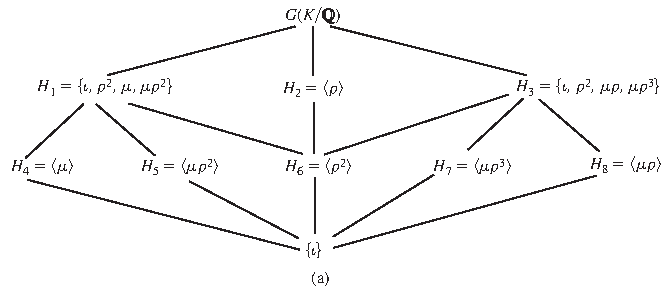
\includegraphics[width=0.917\linewidth,height=.8\textheight,keepaspectratio]{assets/p392_00.pdf}\end{center}
\end{BookFloat}

\begin{BookFloat}{47_illustrations_of_galois_theory-p392-1}
\begin{center}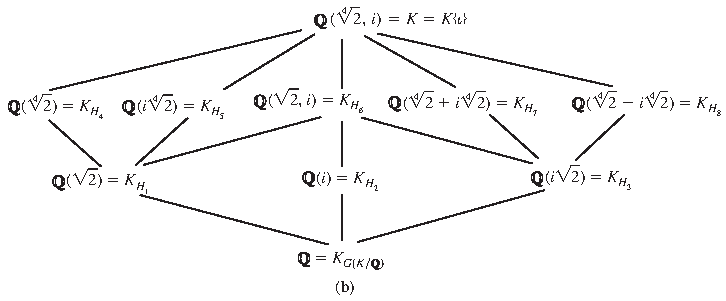
\includegraphics[width=0.995\linewidth,height=.8\textheight,keepaspectratio]{assets/p392_01.pdf}\end{center}
\begin{center}\small\textbf{47.6 Figure}\end{center}
\end{BookFloat}

(a) Group diagram. (b) Field diagram.

\noindent The conjugates of \BookInline{\gamma = \alpha + i\alpha } are thus \BookInline{\alpha + i\alpha,\allowbreak i\alpha - \alpha,\allowbreak - \alpha - i\alpha,\allowbreak } and \BookInline{- i\alpha + \alpha.} Hence

\begin{center}\begin{adjustbox}{max width=\linewidth}\BookInline{\displaystyle \begin{aligned}\;\text{irr}\;(\gamma ,\allowbreak \mathbb{Q})&= [(x- (\alpha + i\alpha ))(x- (i\alpha - \alpha ))] \\ &\cdot [(x- (- \alpha - i\alpha ))(x- (- i\alpha + \alpha ))] \\ &= (x^{2}- 2i\alpha x- 2\alpha ^{2})(x^{2}+ 2i\alpha x- 2\alpha ^{2}) \\ &= x^{4}+ 4\alpha ^{4}= x^{4}+ 8.\end{aligned}}\end{adjustbox}\end{center} \BookEnd{\blacktriangle}

We have seen examples in which the splitting field of a quartic (4th degree) polynomial over a field \BookInline{F} is an extension of \BookInline{F} of degree 8 (Example 47.3) and of degree 24 (Theorem 47.2, with \BookInline{n= 4).} The degree of an extension of a field \BookInline{F} that is a splitting field of a quartic over \BookInline{F} must always divide \BookInline{4!= 24.} The splitting field of \BookInline{(x- 2)^{4}} over \BookInline{\mathbb{Q}} is \BookInline{\mathbb{Q},\allowbreak } an extension of degree 1, and the splitting field of \BookInline{(x^{2}- 2)^{2}} over \BookInline{\mathbb{Q}} is \BookInline{\mathbb{Q}(\sqrt{2}),\allowbreak } an extension of degree 2. Our last example will give an extension of degree 4 for the splitting field of a quartic.

\BookLabel{47.7 Example} Consider the splitting field of \BookInline{x^{4}+ 1} over \BookInline{\mathbb{Q}.} By Theorem 28.12, we can show that \BookInline{x^{4}+ 1} is irreducible over \BookInline{\mathbb{Q},\allowbreak } by arguing that it does not factor in \BookInline{\mathbb{Z}[x].(}See Exercise 1.) The work on complex numbers in Section 3 shows that the zeros of \BookInline{x^{4}+ 1} are \BookInline{(1\pm } \BookInline{i)/\sqrt{2}} and \BookInline{(- 1\pm i)/\sqrt{2}.} A computation shows that if

\begin{center}\begin{adjustbox}{max width=\linewidth}\BookInline{\displaystyle \alpha = { \frac { 1 + i } { \sqrt { 2 } } } ,\allowbreak }\end{adjustbox}\end{center}

\end{BookBody}

% Source PDF page 393; original printed page 376
\BookSource{393}{376}
\BookNarrativetrue

\begin{BookBody}

\noindent then

\begin{center}\begin{adjustbox}{max width=\linewidth}\BookInline{\displaystyle \alpha ^ { 3 } = \frac { - 1 + i } { \sqrt { 2 } } ,\allowbreak  \qquad \alpha ^ { 5 } = \frac { - 1 - i } { \sqrt { 2 } } ,\allowbreak  \qquad \mathrm { a n d } \qquad \alpha ^ { 7 } = \frac { 1 - i } { \sqrt { 2 } } .}\end{adjustbox}\end{center}

\noindent Thus the splitting field \BookInline{K} of \BookInline{x^{4}+ 1} over \BookInline{\mathbb{Q}} is \BookInline{\mathbb{Q}(\alpha ),\allowbreak } and \BookInline{[K:\mathbb{Q}]= 4.} Let us compute \BookInline{G(K/\mathbb{Q})} and give the group and field diagrams. Since there exist automorphisms of \BookInline{K} mapping \BookInline{\alpha } onto each conjugate of \BookInline{\alpha,\allowbreak } and since an automorphism \BookInline{\sigma } of \BookInline{\mathbb{Q}(\alpha )} is completely determined by \BookInline{\sigma (\alpha ),\allowbreak } we see that the four elements of \BookInline{G(K/\mathbb{Q})} are defined by Table 47.8.

\begin{BookFloat}{47_illustrations_of_galois_theory-p393-3}
\begin{center}\small\textbf{47.8 Table}\end{center}
\begin{center}\begin{adjustbox}{max width=\linewidth}
\renewcommand{\arraystretch}{1.2}\setlength{\tabcolsep}{5pt}
\begin{tabular}{c|c|c|c|c}
 & \BookInline{\sigma _{1}} & \BookInline{\sigma _{3}} & \BookInline{\sigma _{5}} & \BookInline{\sigma _{7}}\\\hline
\BookInline{\alpha \to } & \BookInline{\alpha } & \BookInline{\alpha ^{3}} & \BookInline{\alpha ^{5}} & \BookInline{\alpha ^{7}}\\
\end{tabular}
\end{adjustbox}\end{center}
\end{BookFloat}

\noindent Since

\begin{center}\begin{adjustbox}{max width=\linewidth}\BookInline{\displaystyle (\sigma _{j}\sigma _{k})(\alpha )= \sigma _{j}(\alpha ^{k})= (\alpha ^{j})^{k}= \alpha ^{jk}}\end{adjustbox}\end{center}

\noindent and \BookInline{\alpha ^{8}= 1,\allowbreak } we see that \BookInline{G(K/\mathbb{Q})} is isomorphic to the group \BookInline{\{1,\allowbreak 3,\allowbreak 5,\allowbreak 7\}} under multiplication modulo 8. There are only two groups of order 4 up to isomorphism, the cyclic group and the Klein 4-group. Since each element of \BookInline{\{1,\allowbreak 3,\allowbreak 5,\allowbreak 7\}} has order 2 or \BookInline{1,\allowbreak G(K/\mathbb{Q})} is isomorphic with the Klein 4-group. The diagrams are given in Fig. 47.9.

\begin{BookFloat}{47_illustrations_of_galois_theory-p393-7}
\begin{center}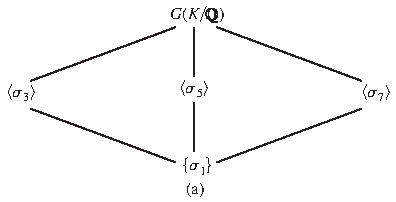
\includegraphics[width=0.543\linewidth,height=.8\textheight,keepaspectratio]{assets/p393_08.pdf}\end{center}
\end{BookFloat}

\begin{BookFloat}{47_illustrations_of_galois_theory-p393-8}
\begin{center}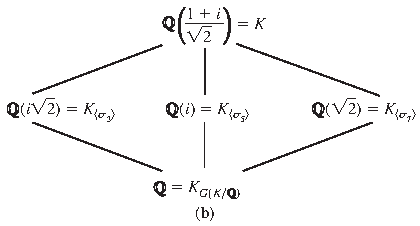
\includegraphics[width=0.576\linewidth,height=.8\textheight,keepaspectratio]{assets/p393_09.pdf}\end{center}
\begin{center}\small\textbf{47.9 Figure}\end{center}
\end{BookFloat}

(a) Group diagram. (b) Field diagram.

To find \BookInline{K_{\langle \sigma _{3}\rangle }}, it is only necessary to find an element of \BookInline{K} not in \BookInline{\mathbb{Q}} fixed by \BookInline{\{\sigma _{1},\allowbreak \sigma _{3}\},\allowbreak } since \BookInline{[K_{\langle \sigma _{3}\rangle }:\mathbb{Q}]= 2.} Clearly \BookInline{\sigma _{1}(\alpha )+ \sigma _{3}(\alpha )} is fixed by both \BookInline{\sigma _{1}} and \BookInline{\sigma _{3},\allowbreak } since \BookInline{\{\sigma _{1},\allowbreak \sigma _{3}\}} \BookInline{= \langle \sigma _{3}\rangle } is a group. We have

\begin{center}\begin{adjustbox}{max width=\linewidth}\BookInline{\displaystyle \sigma _{1}(\alpha )+ \sigma _{3}(\alpha )= \alpha + \alpha ^{3}= i\sqrt{2}.}\end{adjustbox}\end{center}

\noindent Similarly,

\begin{center}\begin{adjustbox}{max width=\linewidth}\BookInline{\displaystyle \sigma _{1}(\alpha )+ \sigma _{7}(\alpha )= \alpha + \alpha ^{7}= \sqrt{2}}\end{adjustbox}\end{center}

\end{BookBody}

% Source PDF page 394; original printed page 377
\BookSource{394}{377}
\BookNarrativetrue

\begin{BookBody}

\noindent is fixed by \BookInline{\langle \sigma _{7}\rangle = \{\sigma _{1},\allowbreak \sigma _{7}\}.} This technique is of no use in finding \BookInline{E_{\langle \sigma _{5}\rangle }}, for

\begin{center}\begin{adjustbox}{max width=\linewidth}\BookInline{\displaystyle \sigma _{1}(\alpha )+ \sigma _{5}(\alpha )= \alpha + \alpha ^{5}= 0,\allowbreak }\end{adjustbox}\end{center}

\noindent and \BookInline{0\in \mathbb{Q}.} But by a similar argument\BookInline{,\allowbreak \sigma _{1}(\alpha )\sigma _{5}(\alpha )} is fixed by both \BookInline{\sigma _{1}} and \BookInline{\sigma _{5},\allowbreak } and

\begin{center}\begin{adjustbox}{max width=\linewidth}\BookInline{\displaystyle \sigma _{1}(\alpha )\sigma _{5}(\alpha )= \alpha \alpha ^{5}= - i.}\end{adjustbox}\end{center}

\noindent Thus \BookInline{\mathbb{Q}(- i)= \mathbb{Q}(i)} is the field we are after. \BookEnd{\blacktriangle}

\end{BookBody}

\BookNarrativefalse

\begin{BookBody}

\BookExerciseTitle{47}

\BookTextHeading{\textbf{Computations (requiring more than the usual amount of theory)}  }

\BookExercise{1.}{Show that \BookInline{x^{4}+ 1} is irreducible in \BookInline{\mathbb{Q}[x],\allowbreak } as we asserted in Example 47.7.}

\BookExercise{2.}{Verify that the intermediate fields given in the field diagram in Fig. 47.6 are correct. (Some are verified in the text. Verify the rest.)}

\BookExercise{3.}{For each field in the field diagram in Fig. 47.6, find a primitive element generating the field over \BookInline{\mathbb{Q}(}see Theorem 45.13) and give its irreducible polynomial over \BookInline{\mathbb{Q}.}}

\BookExercise{4.}{Let \BookInline{\zeta } be a primitive 5th root of unity in \BookInline{\mathbb{C}.}}

\BookExercise{a.}{Show that \BookInline{\mathbb{Q}(\zeta )} is the splitting field of \BookInline{x^{5}- 1} over \BookInline{\mathbb{Q}.}}

\BookExercise{b.}{Show that every automorphism of \BookInline{K= \mathbb{Q}(\zeta )} maps \BookInline{\zeta } onto some power \BookInline{\zeta ^{r}} of \BookInline{\zeta.}}

\BookExercise{c.}{Using part (b), describe the elements of \BookInline{G(K/\mathbb{Q}).}}

\BookExercise{d.}{Give the group and field diagrams for \BookInline{\mathbb{Q}(\zeta )} over \BookInline{\mathbb{Q},\allowbreak } computing the intermediate fields as we did in Examples 47.3 and 47.7.}

\BookExercise{5.}{Describe the group of the polynomial \BookInline{(x^{5}- 2)\in (\mathbb{Q}(\zeta ))[x]} over \BookInline{\mathbb{Q}(\zeta ),\allowbreak } where \BookInline{\zeta } is a primitive 5th root of unity.}

\BookExercise{6.}{Repcat Exercise 4 for \BookInline{\zeta } a primitive 7th root of unity in \BookInline{\mathbb{C}.}}

\BookExercise{7.}{In the easiest way possible, describe the group of the polynomial}

\begin{center}\begin{adjustbox}{max width=\linewidth}\BookInline{\displaystyle (x^{8}- 1)\in \mathbb{Q}[x]}\end{adjustbox}\end{center}

\noindent over \BookInline{\mathbb{Q}.}

\BookExercise{8.}{Find the splitting field \BookInline{K} in \BookInline{\mathbb{C}} of the polynomial \BookInline{(x^{4}- 4x^{2}- 1)\in \mathbb{Q}[x].} Compute the group of the polynomial over \BookInline{\mathbb{Q}} and exhibit the correspondence between the subgroups of \BookInline{G(K/\mathbb{Q})} and the intermediate fields. In other words, do the complete job.}

\BookExercise{9.}{Express each of the following symmetric functions in \BookInline{y_{1},\allowbreak y_{2},\allowbreak y_{3}} over \BookInline{\mathbb{Q}} as a rational function of the elementary symmetric functions \BookInline{s_{1},\allowbreak s_{2},\allowbreak s_{3}.}}

\BookExercise{a.}{\textbf{a}\BookInline{.y_{1}^{2}+ y_{2}^{2}+ y_{3}^{2}}}

\noindent \textbf{b.} \BookInline{\frac{y_{1}}{y_{2}}+\frac{y_{2}}{y_{1}}+\frac{y_{1}}{y_{3}}+\frac{y_{3}}{y_{1}}+\frac{y_{2}}{y_{3}}+\frac{y_{3}}{y_{2}}}

\BookExercise{10.}{Let \BookInline{\alpha _{1},\allowbreak \alpha _{2},\allowbreak \alpha _{3}} be the zeros in \BookInline{\mathbb{C}} of the polynomial}

\begin{center}\begin{adjustbox}{max width=\linewidth}\BookInline{\displaystyle (x^{3}- 4x^{2}+ 6x- 2)\in \mathbb{Q}[x].}\end{adjustbox}\end{center}

\noindent Find the polynomial having as zeros precisely the following:

\BookExercise{a.}{\textbf{a}\BookInline{.\alpha _{1}+ \alpha _{2}+ \alpha _{3}}}

\BookExercise{b.}{\textbf{b}\BookInline{.\alpha _{1}^{2},\allowbreak \alpha _{2}^{2},\allowbreak \alpha _{3}^{2}}}

\BookTextHeading{\textbf{Theory}}

\BookExercise{11.}{Show that every finite group is isomorphic to some Galois group \BookInline{G(K/F)} for some finite normal extension \BookInline{K} of some field \BookInline{F.}}

\end{BookBody}

% Continuation on source PDF page 395, preceding Section 48
\BookNarrativefalse

\begin{BookBody}

\BookExercise{12.}{Let \BookInline{f(x)\in F[x]} be a monic polynomial of degree \BookInline{n} having all its irreducible factors separable over \BookInline{F.} Let \BookInline{K} be the splitting field of \BookInline{f(x)} over \BookInline{F,\allowbreak } and suppose that \BookInline{f(x)} factors in \BookInline{K[x]} into}

\begin{center}\begin{adjustbox}{max width=\linewidth}\BookInline{\displaystyle \prod _{i= 1}^{n}(x- \alpha _{i}).}\end{adjustbox}\end{center}

Let

\begin{center}\begin{adjustbox}{max width=\linewidth}\BookInline{\displaystyle \Delta (f)= \prod _{i<j}(\alpha _{i}- \alpha _{j});}\end{adjustbox}\end{center}

the product \BookInline{(\Delta (f))^{2}} is the\textbf{ discriminant of} \BookInline{f(x).}

\BookExercise{a.}{Show that \BookInline{\Delta (f)= 0} if and only if \BookInline{f(x)} has as a factor the square of some irreducible polynomial in \BookInline{F[x].}}

\BookExercise{b.}{Show that \BookInline{(\Delta (f))^{2}\in F.}}

\BookExercise{c.}{\textbf{c}\BookInline{.G(K/F)} may be viewed as a subgroup of \BookInline{\overline{S_{n}},\allowbreak } where \BookInline{\overline{S_{n}}} is the group of all permutations of \BookInline{\{\alpha _{i}\mid i= 1,\allowbreak \cdots,\allowbreak n\}.} Show that \BookInline{G(K/F),\allowbreak } when viewed in this fashion, is a subgroup of \BookInline{\overline{A_{n}},\allowbreak } the group formed by all even permutations of \BookInline{\{\alpha _{i}\mid i= 1,\allowbreak \cdots,\allowbreak n\},\allowbreak } if and only if \BookInline{\Delta (f)\in F.}}

\BookExercise{13.}{An element of \BookInline{\mathbb{C}} is an\textbf{ algebraic integer} if it is a zero of some\textit{ monic} polynomial in \BookInline{\mathbb{Z}[x].} Show that the set of all algebraic integers forms a subring of \BookInline{\mathbb{C}.}}

\end{BookBody}
\ifdefined\BookMaster\let\BookFinish\relax\else\def\BookFinish{\end{document}}\fi\BookFinish
